% BEGIN PREAMBEL
\documentclass[9pt]{beamer}
\usepackage[british]{babel}
\usepackage[latin1]{inputenc}
\usepackage{multimedia}
\usepackage{amsmath,amsfonts,amssymb}
\usepackage{upgreek}
\usepackage{pgfpages}
\usepackage[version=3]{mhchem}
\usepackage{lmodern}
\usepackage{graphicx}
\usepackage{multicol}
\usepackage{xcolor}
\usepackage{wrapfig}
\usepackage{siunitx}
\newcommand{\as}{\\[14pt]}
\newcommand{\s}{\\[7pt]}
\newcommand{\is}{\\[2pt]}
\newcommand{\no}{\noindent}
\newcommand{\ka}{\hspace*{0.5cm}}
\newcommand{\ma}{\hspace*{1cm}}
\newcommand{\ga}{\hspace*{1.5cm}}
\newcommand{\li}{\left|}
\newcommand{\re}{\right|}
\newcommand{\const}{\text{const.}}
\newcommand{\z}{\text}
\newcommand{\terminal}[1]{\colorbox{black}{\textcolor{white}{{\fontfamily{phv}\selectfont \scriptsize{#1}}}}}
\newcommand{\plugin}[1]{\textit{\flq#1\frq}}
\usetheme{Boadilla}
\graphicspath{ {Pics/} }
\usecolortheme{beaver}
\useoutertheme{miniframes}
\beamertemplatenavigationsymbolsempty
\makeindex
\title[Analysis]{Discussion of the Pad Analysis}
\author[M. Reichmann]{Michael Reichmann}
\institute[\textbf{\textit{ETH}}\scalebox{.6}{\textit{Z\"{u}rich}}]{Swiss Federal Institute of Technology Zurich}
% END PREAMBEL
\begin{document}
% ============================
% BEGIN TITLE PAGE
% ============================
\begin{frame}
	\begin{center}
		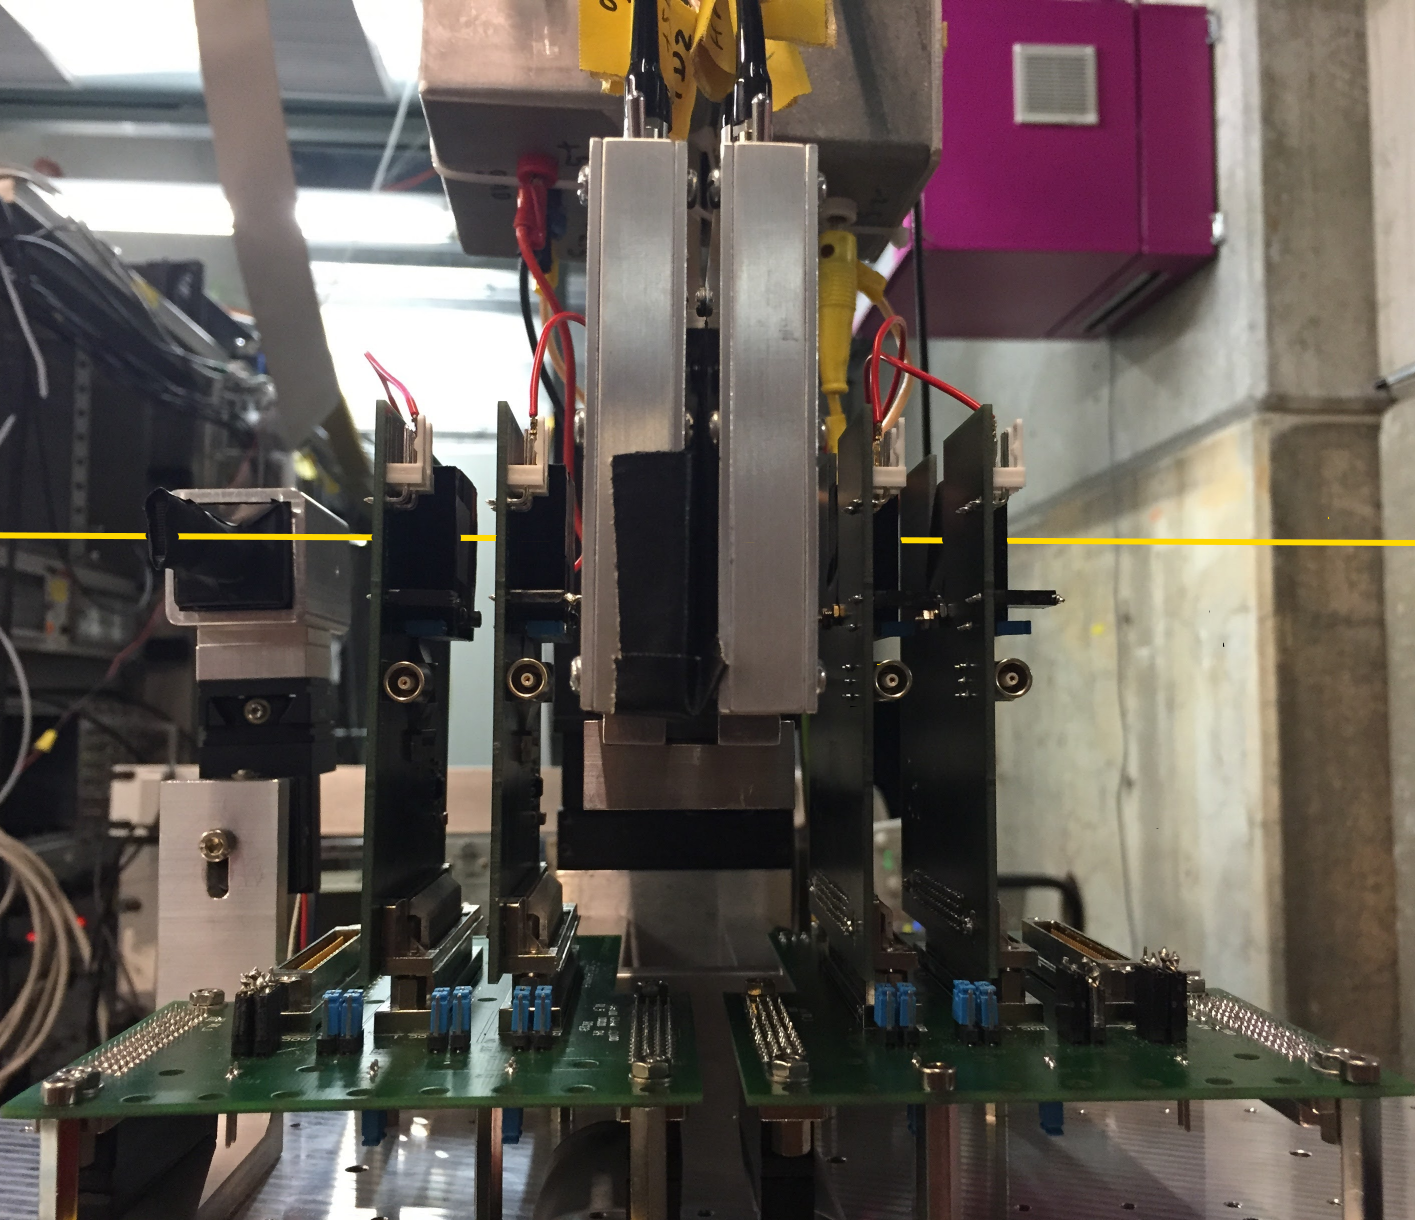
\includegraphics[width=4cm]{telescope3}
	\end{center}
	\begin{alertblock}{
		\begin{center}
			\textbf{Meeting \today}
		\end{center}}
		\vspace*{10pt}
		\begin{center}\small
		Michael Reichmann
		\end{center}\normalsize
	\end{alertblock}
\end{frame}
% END
% ============================
% BEGIN TABLE OF CONTENTS
% ============================
\begin{frame}[allowframebreaks]
	\frametitle{Table of contents}
	\tableofcontents[pausesections]
\end{frame}
% END
% ====================================================================================
% INTRO
% ====================================================================================
\section{Introduction}
\begin{frame}
	\begin{center}
		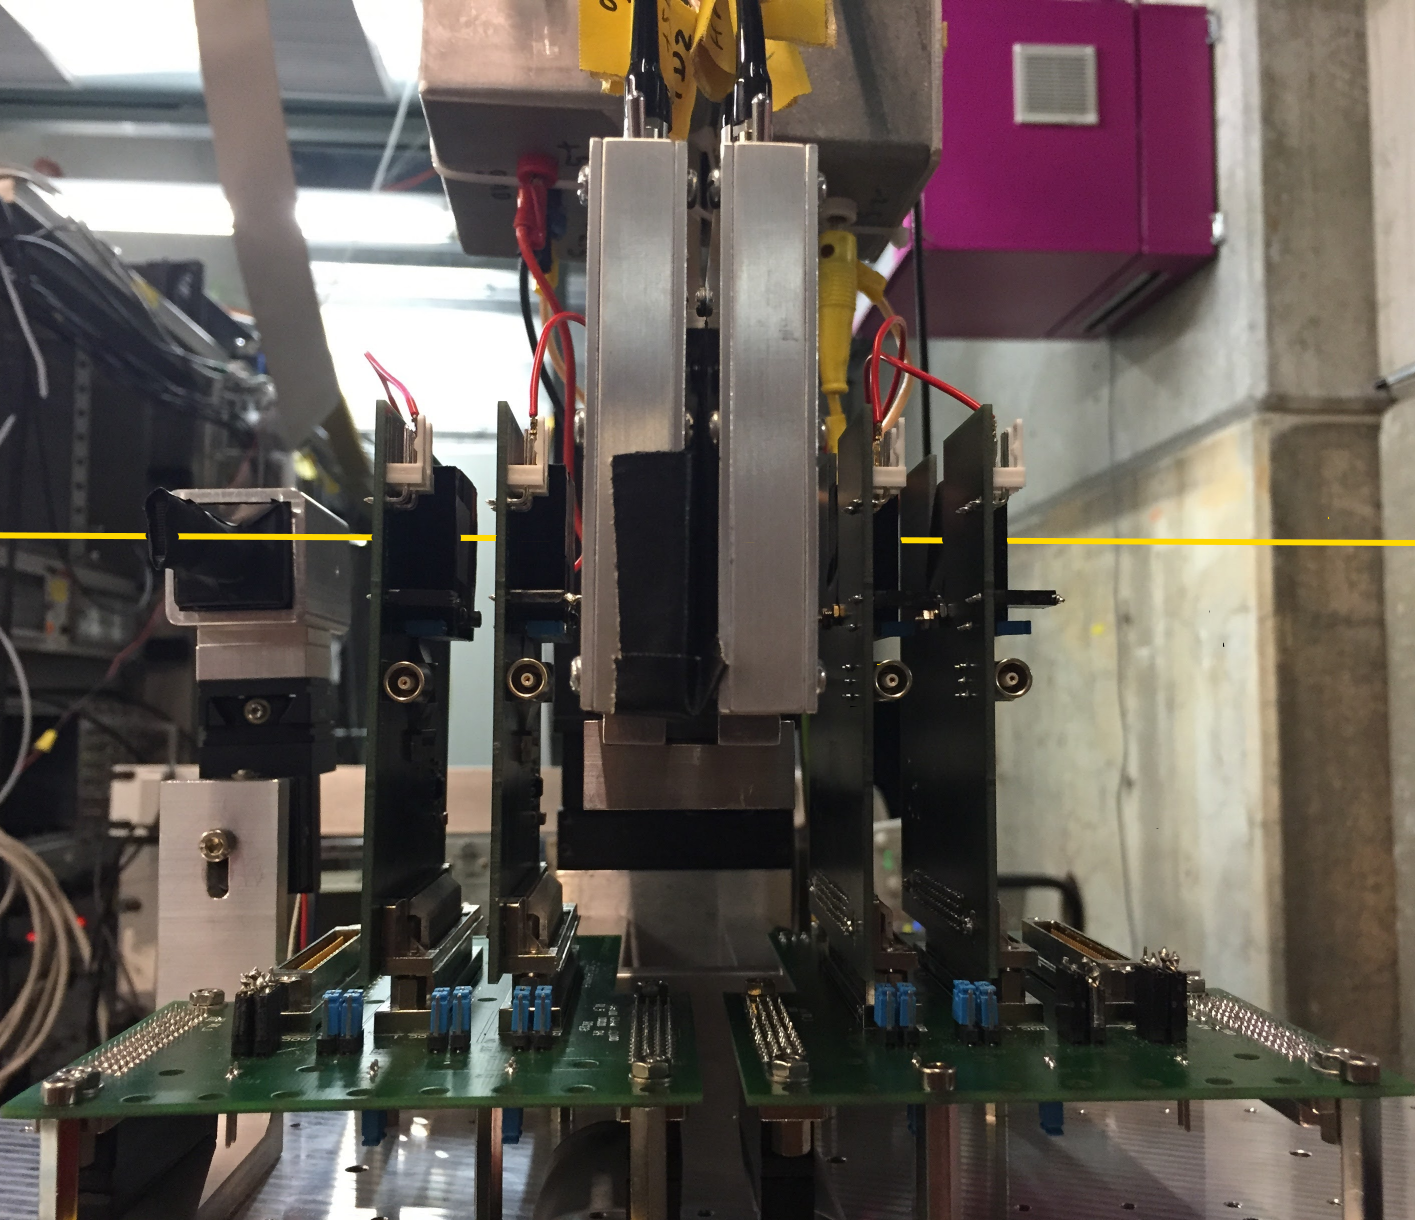
\includegraphics[width=6cm]{telescope3}
	\end{center}
\end{frame}
% new frame ============================
\begin{frame}
	\begin{center}
		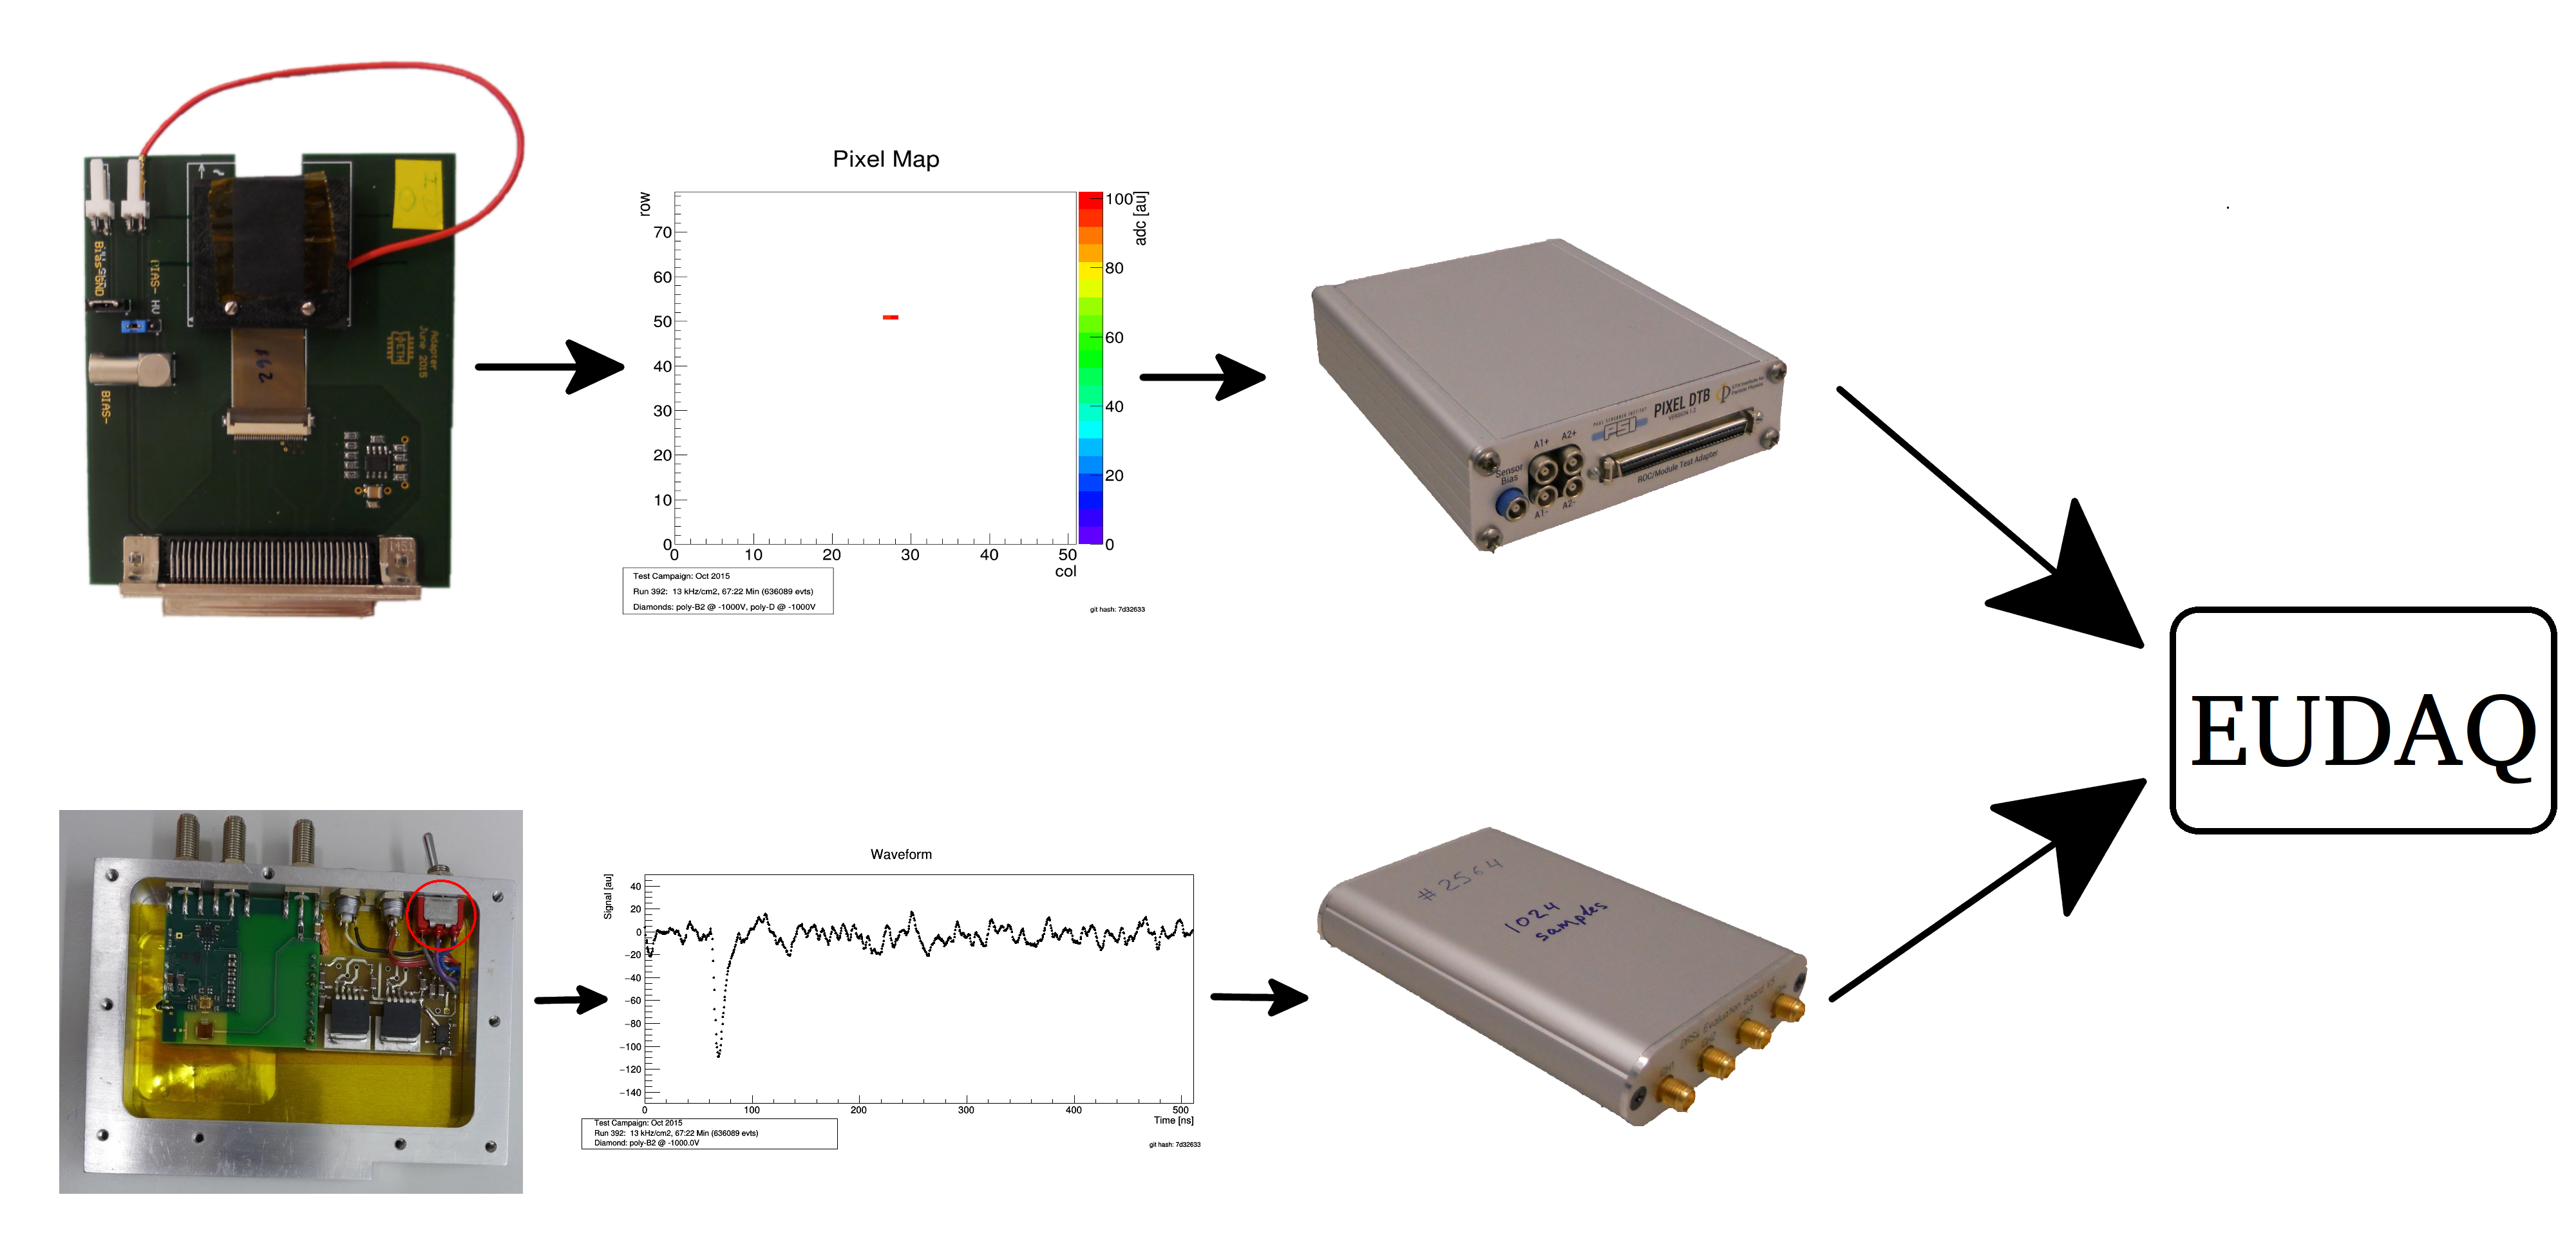
\includegraphics[width=\textwidth]{Intro}
	\end{center}
	\begin{itemize}
		\item EUDAQ saves event based data stream as binary file
		\item require conversion to readable data
	\end{itemize}
\end{frame}
% ====================================================================================
% ====================================================================================
% CONVERTER
% ====================================================================================
\section{EUDAQ Converter}
\subsection{Waveforms}
\begin{frame}
\end{frame}
% ====================================================================================
\subsection{Definition of the Peakfinding Regions}
\begin{frame}
\end{frame}
% ====================================================================================
\subsection{Definition of the Integral Ranges}
\begin{frame}
\end{frame}
% ====================================================================================
% TELESCOPE ANALYSIS
% ====================================================================================
\section{Telescope Analysis}
\subsection{Tracks}
\begin{frame}
\end{frame}
% ====================================================================================
\subsection{$\upchi^{2}$}
\begin{frame}
\end{frame}
% ====================================================================================
\subsection{Track Angle}
\begin{frame}
\end{frame}
% ====================================================================================
% CUTS
% ====================================================================================
\section{Cuts}
\subsection{Tracks}
\begin{frame}
\end{frame}
% ====================================================================================
\subsection{Signal}
\begin{frame}
\end{frame}
% ====================================================================================
% PAD ANALYSIS
% ====================================================================================
\section{Diamond Pad Analysis}
\subsection{Pedestal}
\begin{frame}
\end{frame}
% ====================================================================================
\subsection{Pedestal}
\begin{frame}
\end{frame}
% ====================================================================================
\subsection{Signal}
\begin{frame}
\end{frame}
% ====================================================================================
\subsection{Pulser}
\begin{frame}
\end{frame}
% ====================================================================================
\subsection{Beam Profile}
\begin{frame}
\end{frame}
% ====================================================================================
\subsection{Signal Peak Positions in Time}
\begin{frame}
\end{frame}
% ====================================================================================
\subsection{2D Signal Maps}
\begin{frame}
\end{frame}
% ====================================================================================
\subsection{Diamond Currents}
\begin{frame}
\end{frame}

% ============================
% DOCUMENT END
\end{document}

